
\documentclass{PoS}
\usepackage{amsmath}

\title{Single top quark production in CMS}

\ShortTitle{Single top quark production in CMS}

\author{
    \speaker{Matthias Komm}, on behalf of the CMS collaborations\\
    Imperial College London (UK)\\
    E-mail: \email{Matthias.Komm@cern.ch}
}

\abstract{
In this note, latest cross section measurements of single top quark production in the three main production modes, $s$~channel, W-associated, and $t$~channel, by the CMS collaboration are presented. For the measurements proton-proton collision data at centre-of-mass energies of 7, 8, and 13~TeV have been analysed.
}

\FullConference{
    39th International Conference on High Energy Physics (ICHEP)\\
    04-11 July, 2018\\
    Seoul, Korea
}

\begin{document}

\section{Introduction}
Single top quark production processes are excellent probes to test the predictions of electroweak interactions at the scale of the top quark mass and beyond. Inclusive single top quark cross section measurements can be used to infer the absolute value of the CKM matrix element $\mathrm{V}_\mathrm{tb}$ in a model-independent manner whereas  ratios of top quark over antiquark production cross sections are sensitive to the parton distribution function (PDF). In the following recent measurements of single top quark production via the $s$~channel, W-associated, and $t$~channel are presented.

\section{\textit{s}~channel}

The single top quark $s$-channel production mode has the smallest cross section amongst the three processes. It has been measured using pp collision data recorded by the CMS experiment at centre-of-mass energies of 7 and 8~TeV~\cite{sch}. Events containing one isolated electron or muon and two or three jets of which one or two are b-tagged have been analysed. By performing a simultaneous maximum likelihood (ML) fit to the distribution of a Boosted Decision Tree (BDT) discriminant a signal strength of $\sigma^\mathrm{meas.}_{s\mbox{-}\mathrm{ch.}}/\sigma^\mathrm{theo.}_{s\mbox{-}\mathrm{ch.}}=2.0\pm0.9$ is obtained. This result corresponds to an observed (expected) significance of 2.5 (1.1) standard deviations.

%\begin{figure}[!htb]
%\begin{center}
%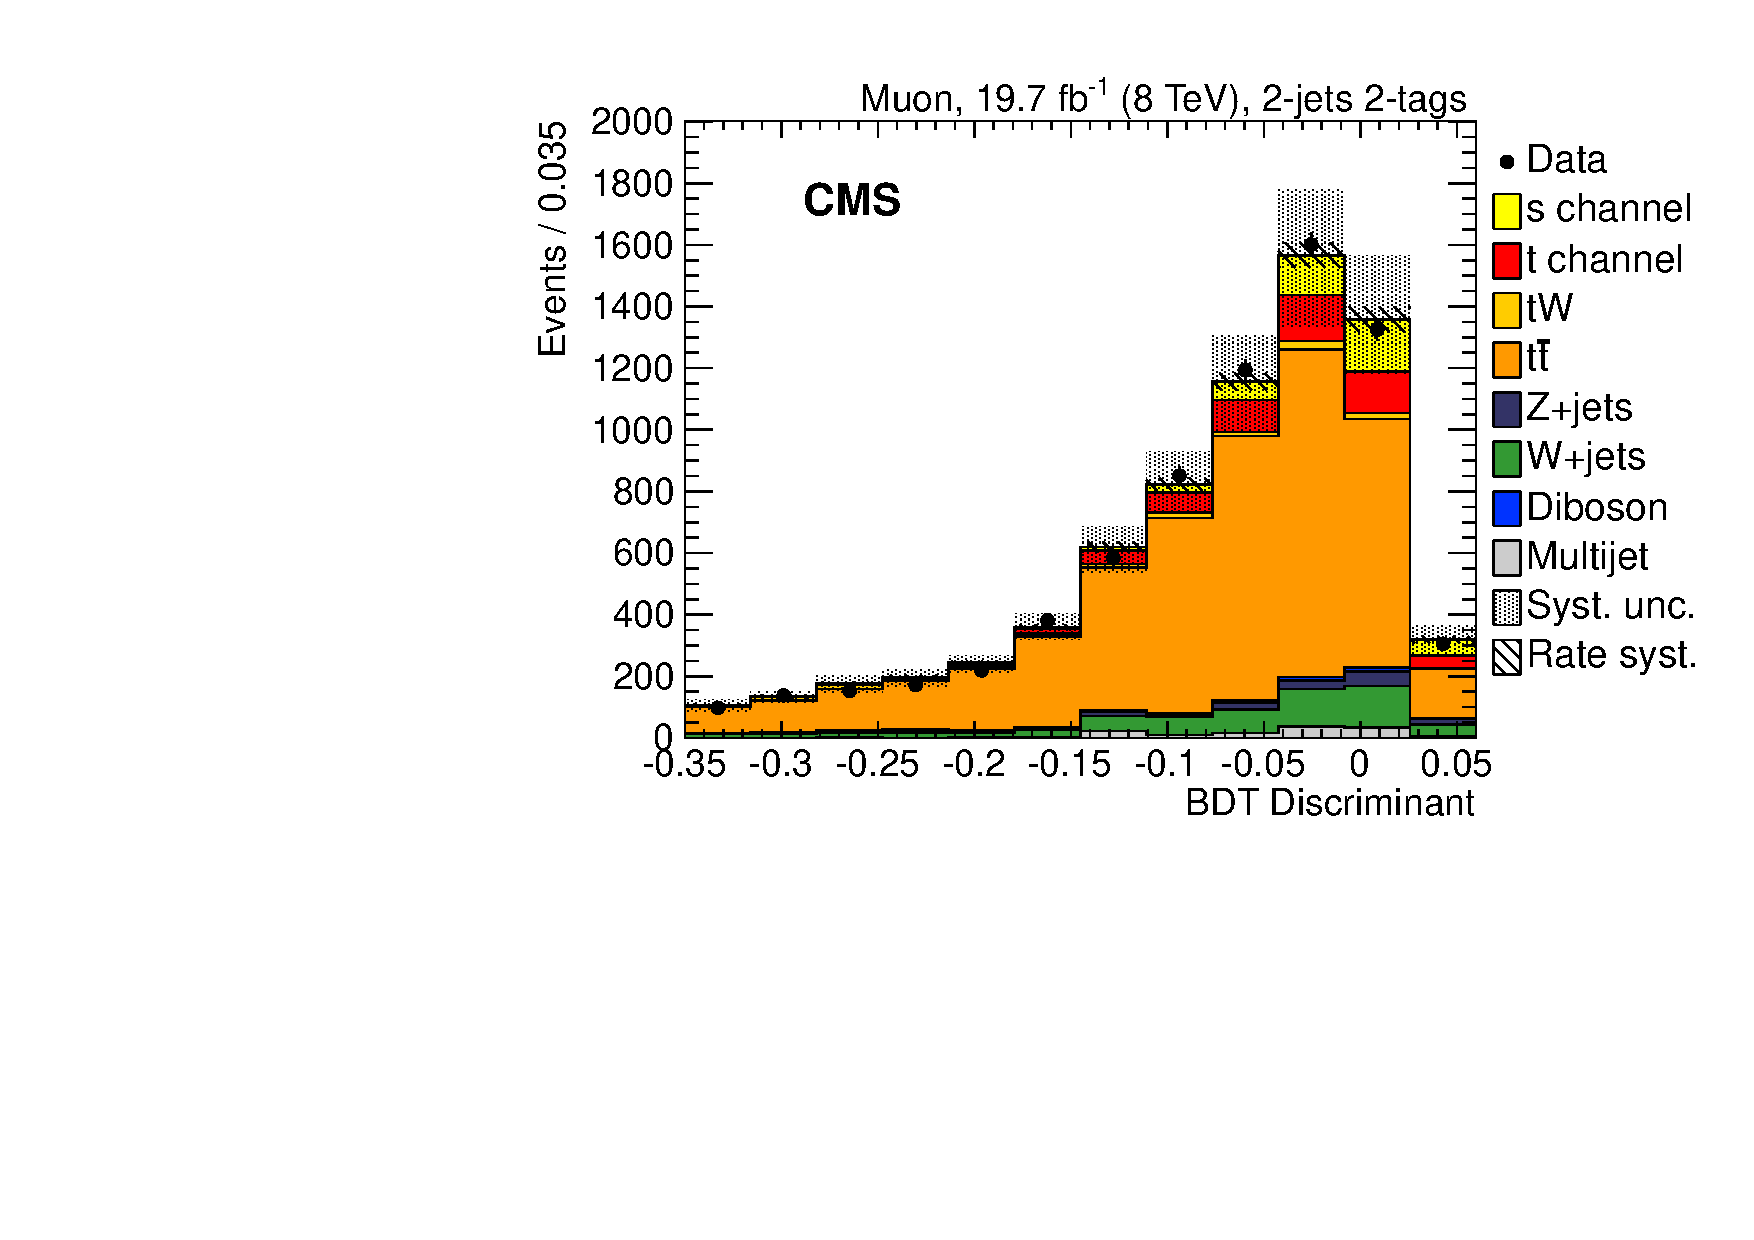
\includegraphics[width=0.48\textwidth]{sch1.pdf}\hspace{0.02\textwidth}
%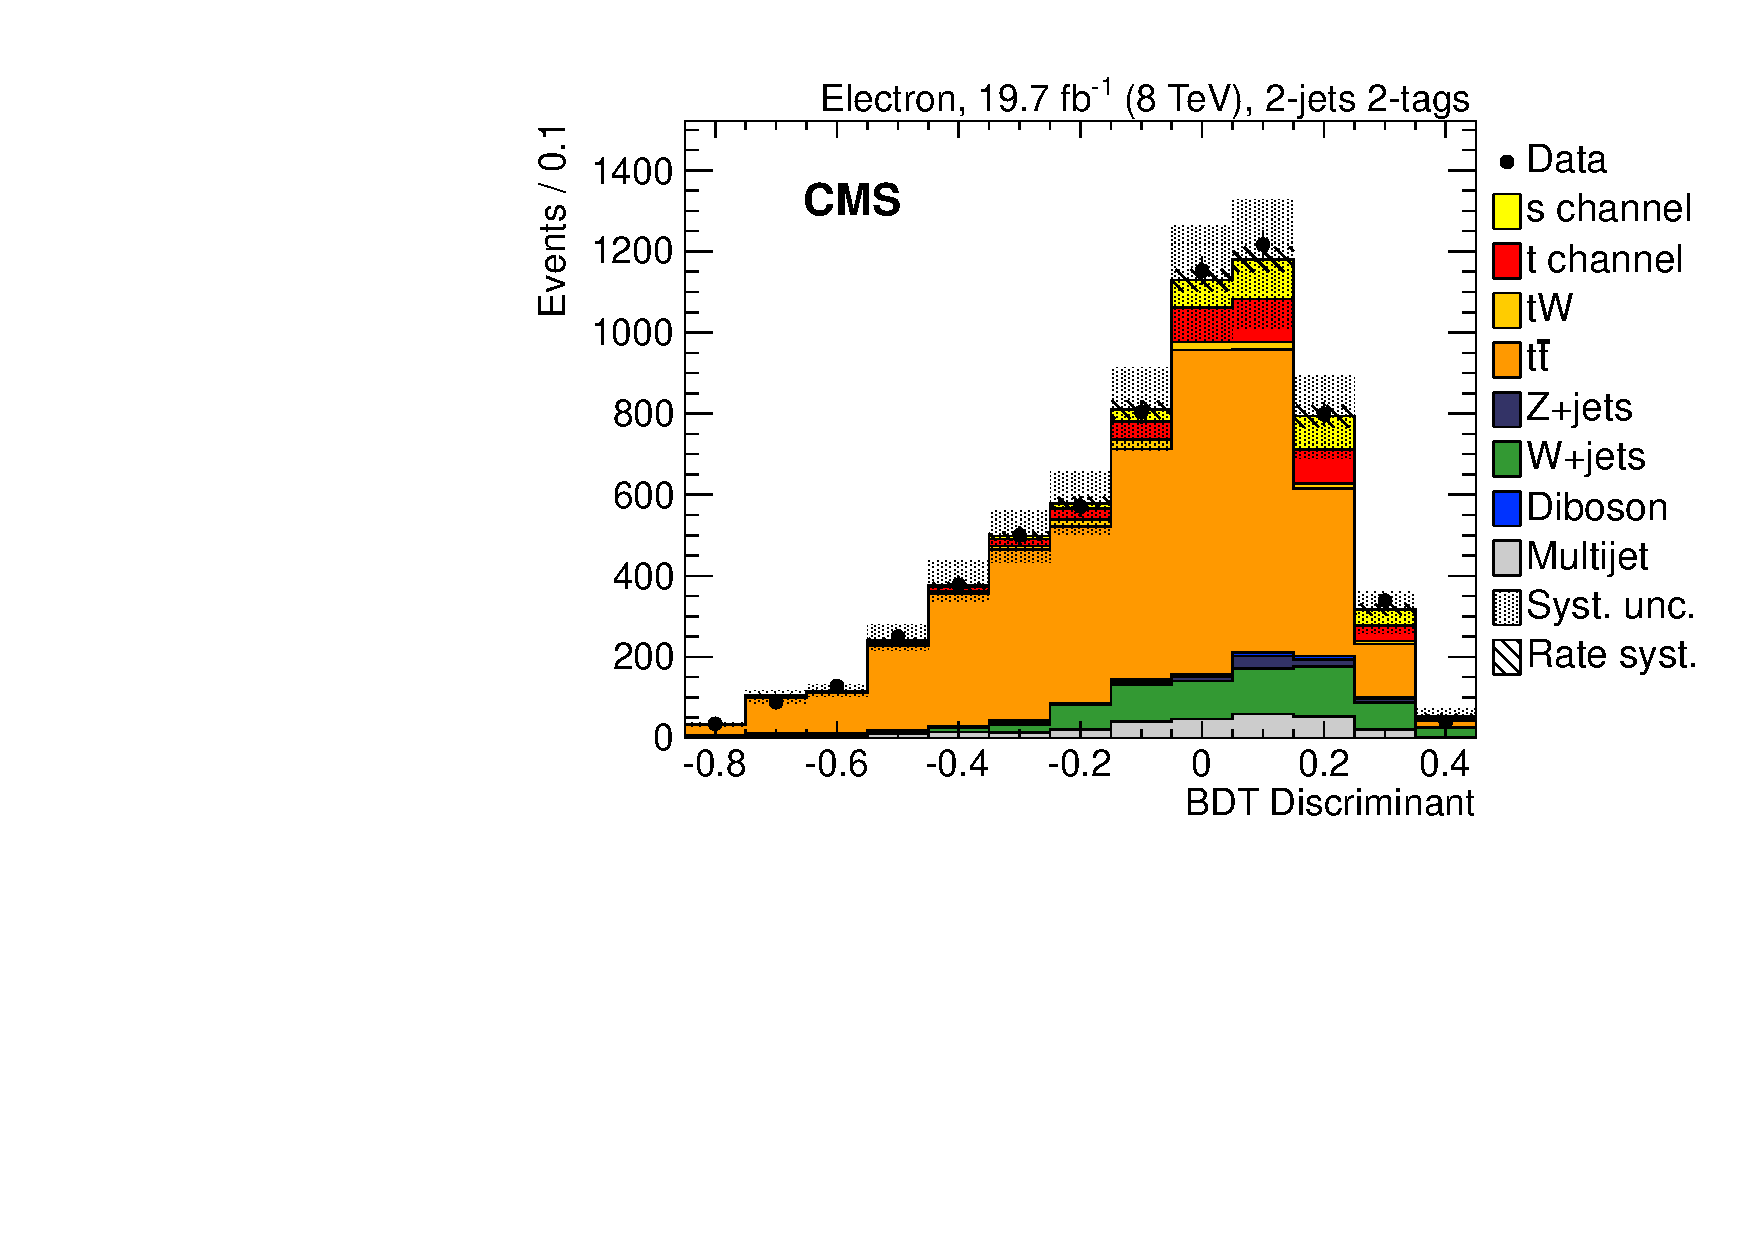
\includegraphics[width=0.48\textwidth]{sch2.pdf}
%\caption{\label{fig:s-channel-bdt}Ref.~\cite{sch}.}
%\end{center}
%\end{figure}

\section{W-associated production}

The cross section of producing a single top quark in association with a W~boson has been measured at 13~TeV in events containing one isolated muon and one isolated electron together with one or two jets~\cite{tWch}. The signal yield is estimated by performing a ML fit to the distributions of a BDT discriminant in 1j1b and 2j1b regions (shown in Fig.~\ref{fig:tw-channel-bdt}) and to the transverse momentum of the subleading jet in the 2j2b control region where the latter allows an in-situ constraint of the jet energy calibration uncertainty. A cross section of $63.1\pm1.8~\mathrm{(stat)}\pm6.4~\mathrm{(syst)}\pm2.1~\mathrm{(lumi)}~\mathrm{pb}$ is found which agrees well with the predicted cross section of $71.7\pm1.8~\mathrm{(scale)}\pm3.4~\mathrm{(PDF)}~\mathrm{pb}$ calculated at approximate next-to-next-to-leading order~\cite{tw-xsec}.

\begin{figure}[!htb]
\begin{center}
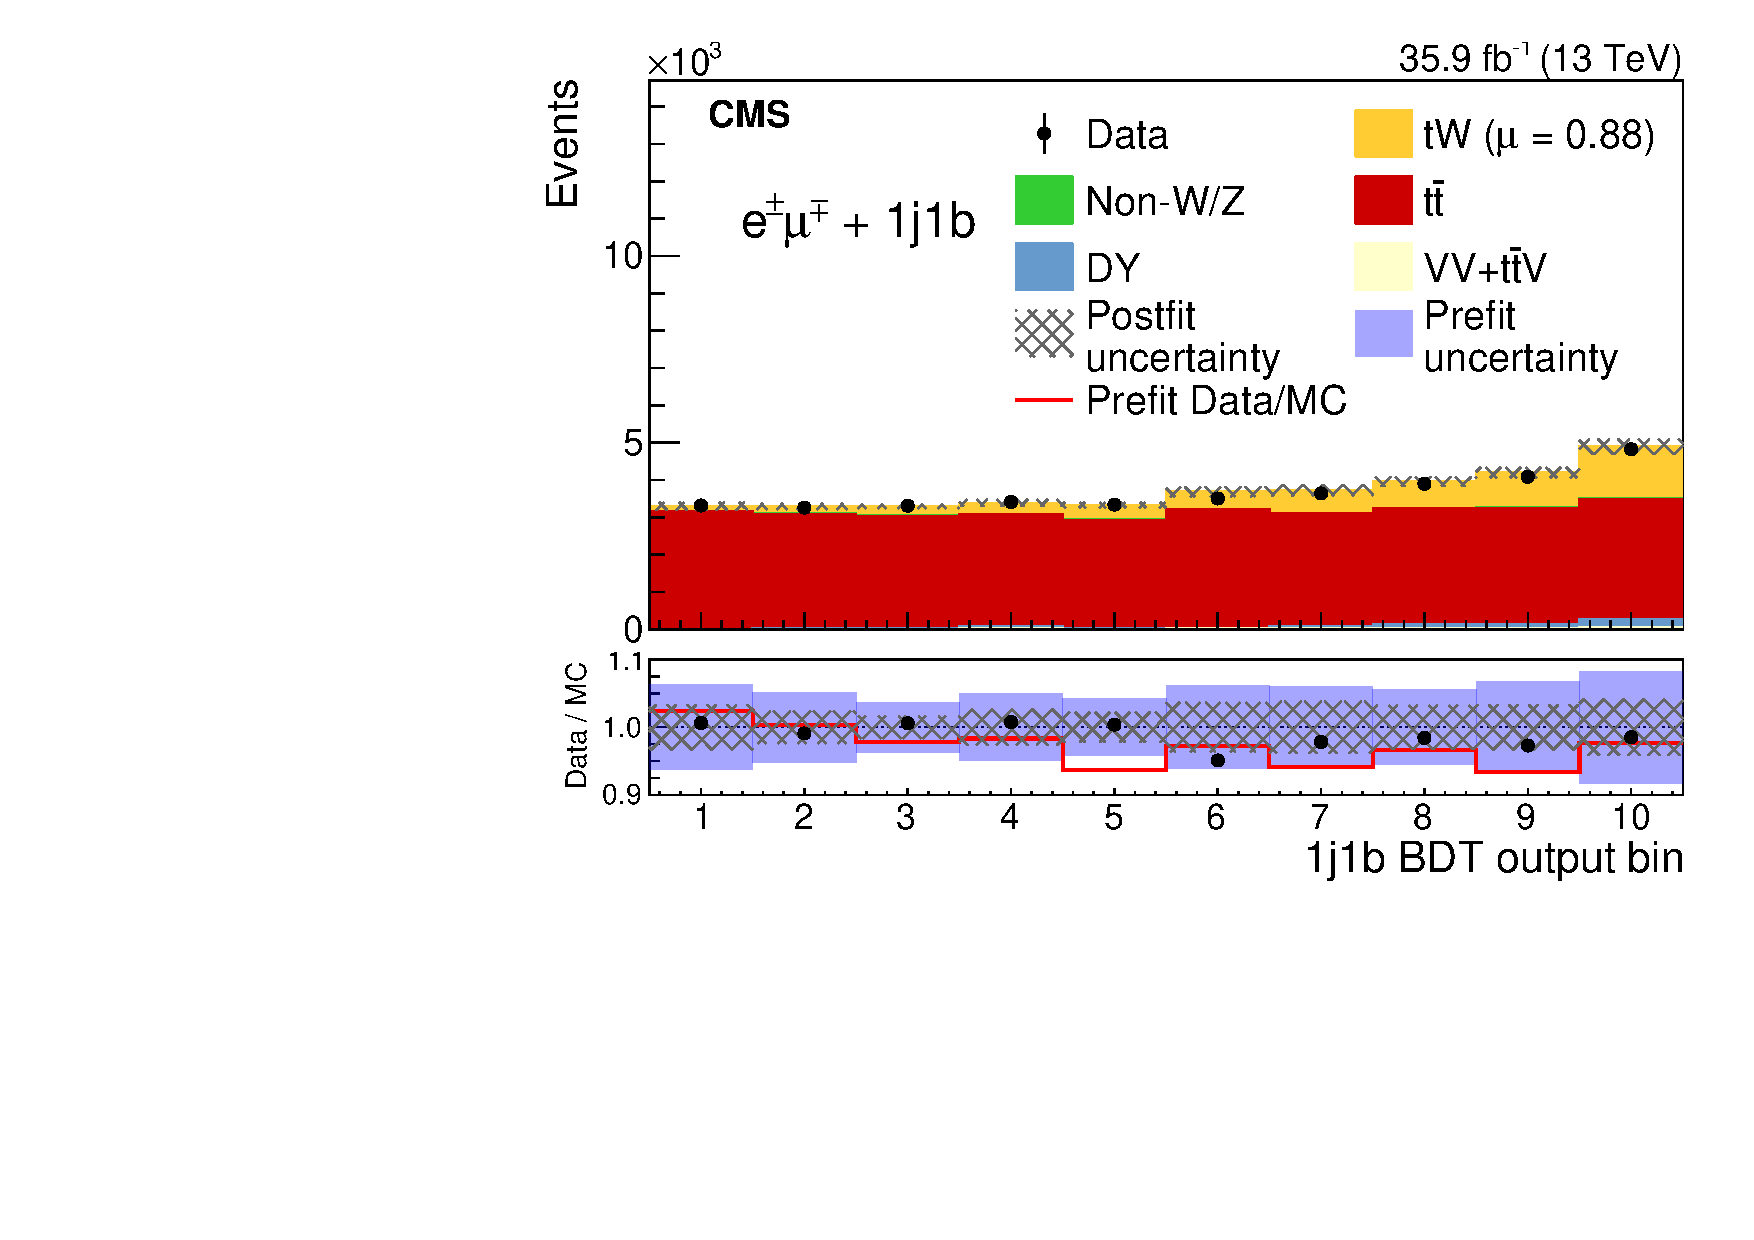
\includegraphics[width=0.48\textwidth]{tw2.pdf}\hspace{0.02\textwidth}
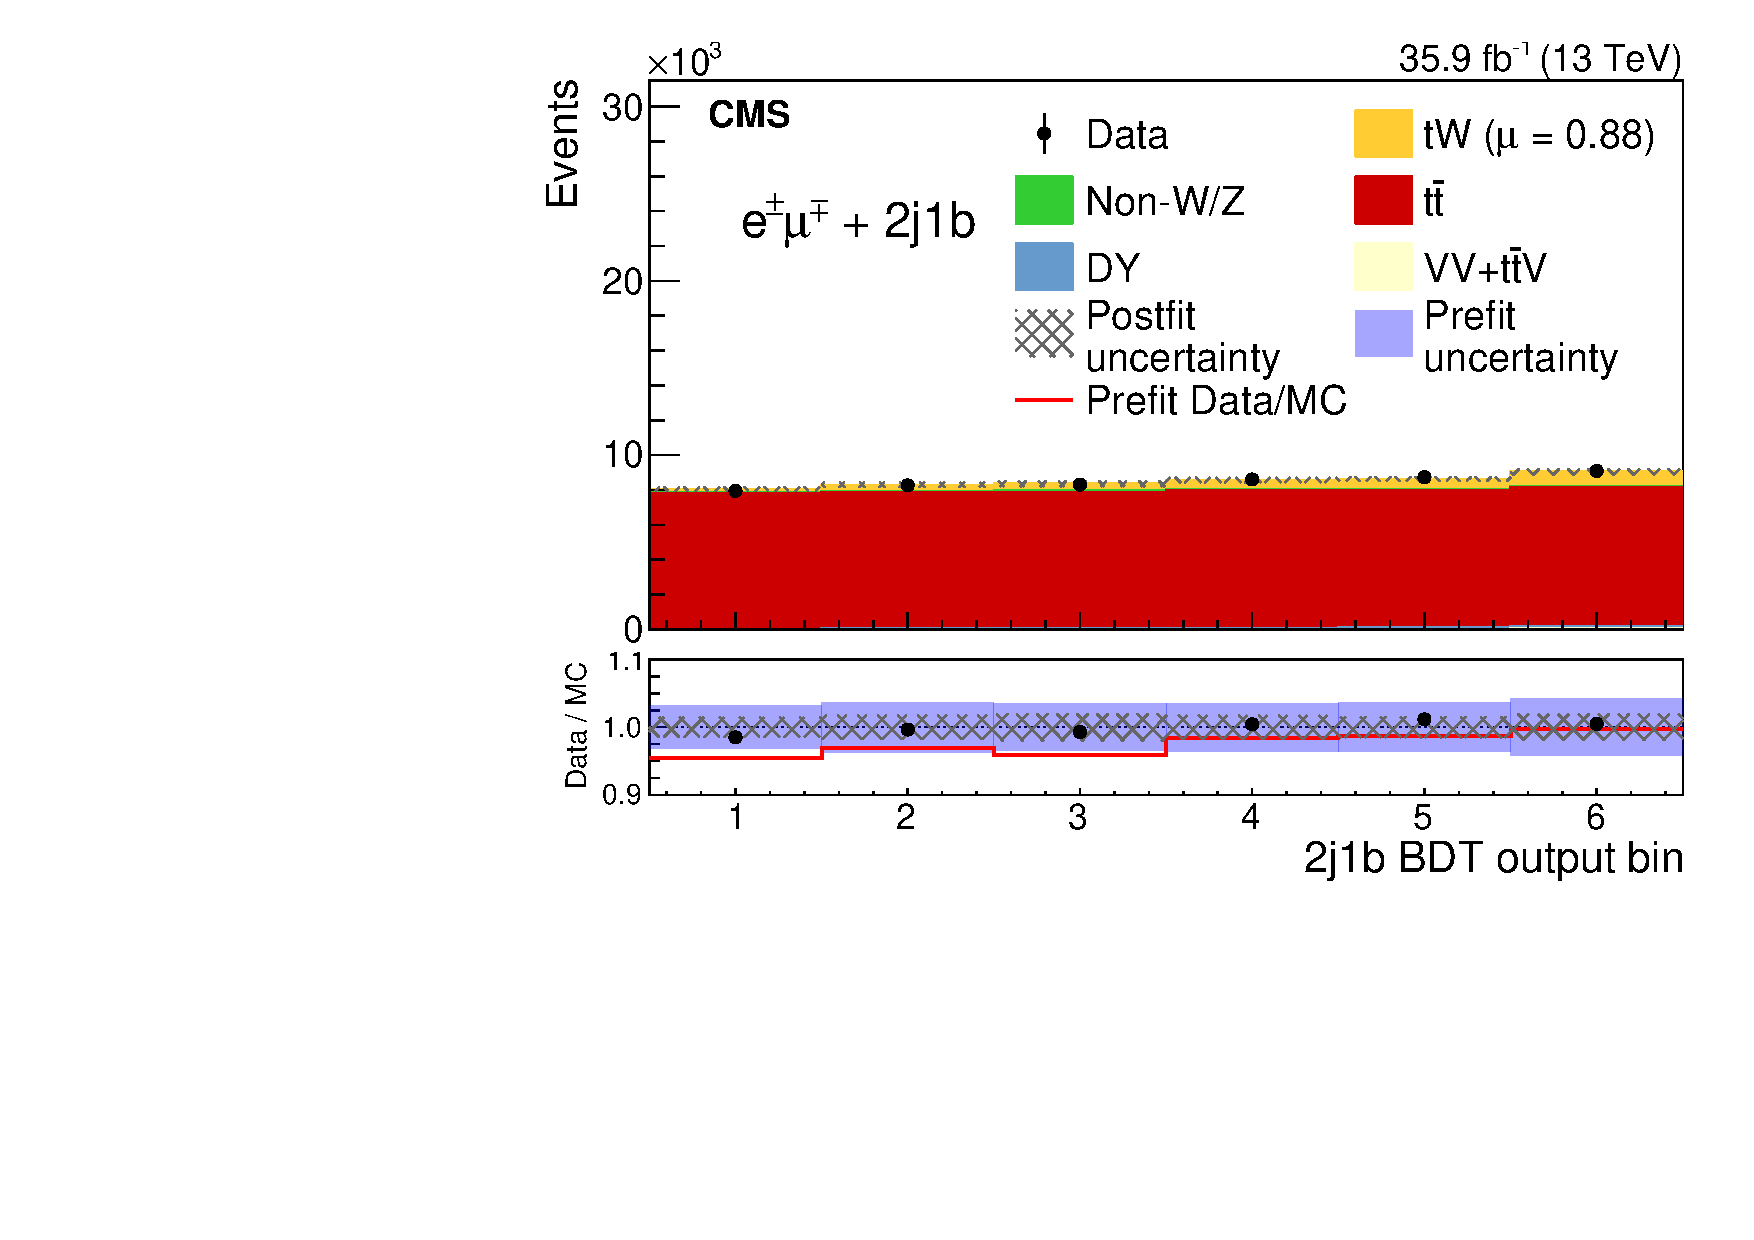
\includegraphics[width=0.48\textwidth]{tw3.pdf}
\caption{\label{fig:tw-channel-bdt}Distributions of a BDT discriminant in (left)~1j1b and (right)~2j1b regions used to estimate the W-associated single top quark cross section at 13~TeV. The figures are taken from Ref.~\cite{tWch}.}
\end{center}
\end{figure}

\section{\textit{t}~channel}

The production of single top quarks via the $t$~channel does not occur charge-symmetric in pp collisions. The charge ratio, $R=\sigma_{t\mbox{-}\mathrm{ch.}}({\mathrm{t}})/\sigma_{t\mbox{-}\mathrm{ch.}}({\bar{\mathrm{t}}})$, depends on the valence quark composition of the proton since an up quark in the initial state leads to the production of a top quark whereas a down quark would yield a top antiquark instead. A corresponding analysis~\cite{tch} is performed using pp collision data at 13~TeV. Events containing an isolated muon or electron together with two or three jets of which one or two are b-tagged are analysed. The distributions of a BDT discriminant for top quark and antiquark events are used to infer the charge ratio through a simultaneous ML fit while allowing for potential cancellations of systematic uncertainties. A charge ratio of $R=1.65\pm0.02~\mathrm{(stat)}\pm0.04~\mathrm{(syst)}$ is found and compared in Fig.~\ref{fig:t-channel-ratio} to the predictions of various PDF sets. The inclusive cross section in $t$~channel has been measured as well and found to be $219.0\pm1.5~\mathrm{(stat)}\pm33.0~\mathrm{(syst)}~\mathrm{pb}$ which is well in agreement with the next-to-leading order prediction of $217.0^{+9.0}_{-7.7}~\mathrm{(scale+PDF+\alpha_s)}~\mathrm{pb}$~\cite{hathor}.
 
%\begin{figure}[!htb]
%\begin{center}
%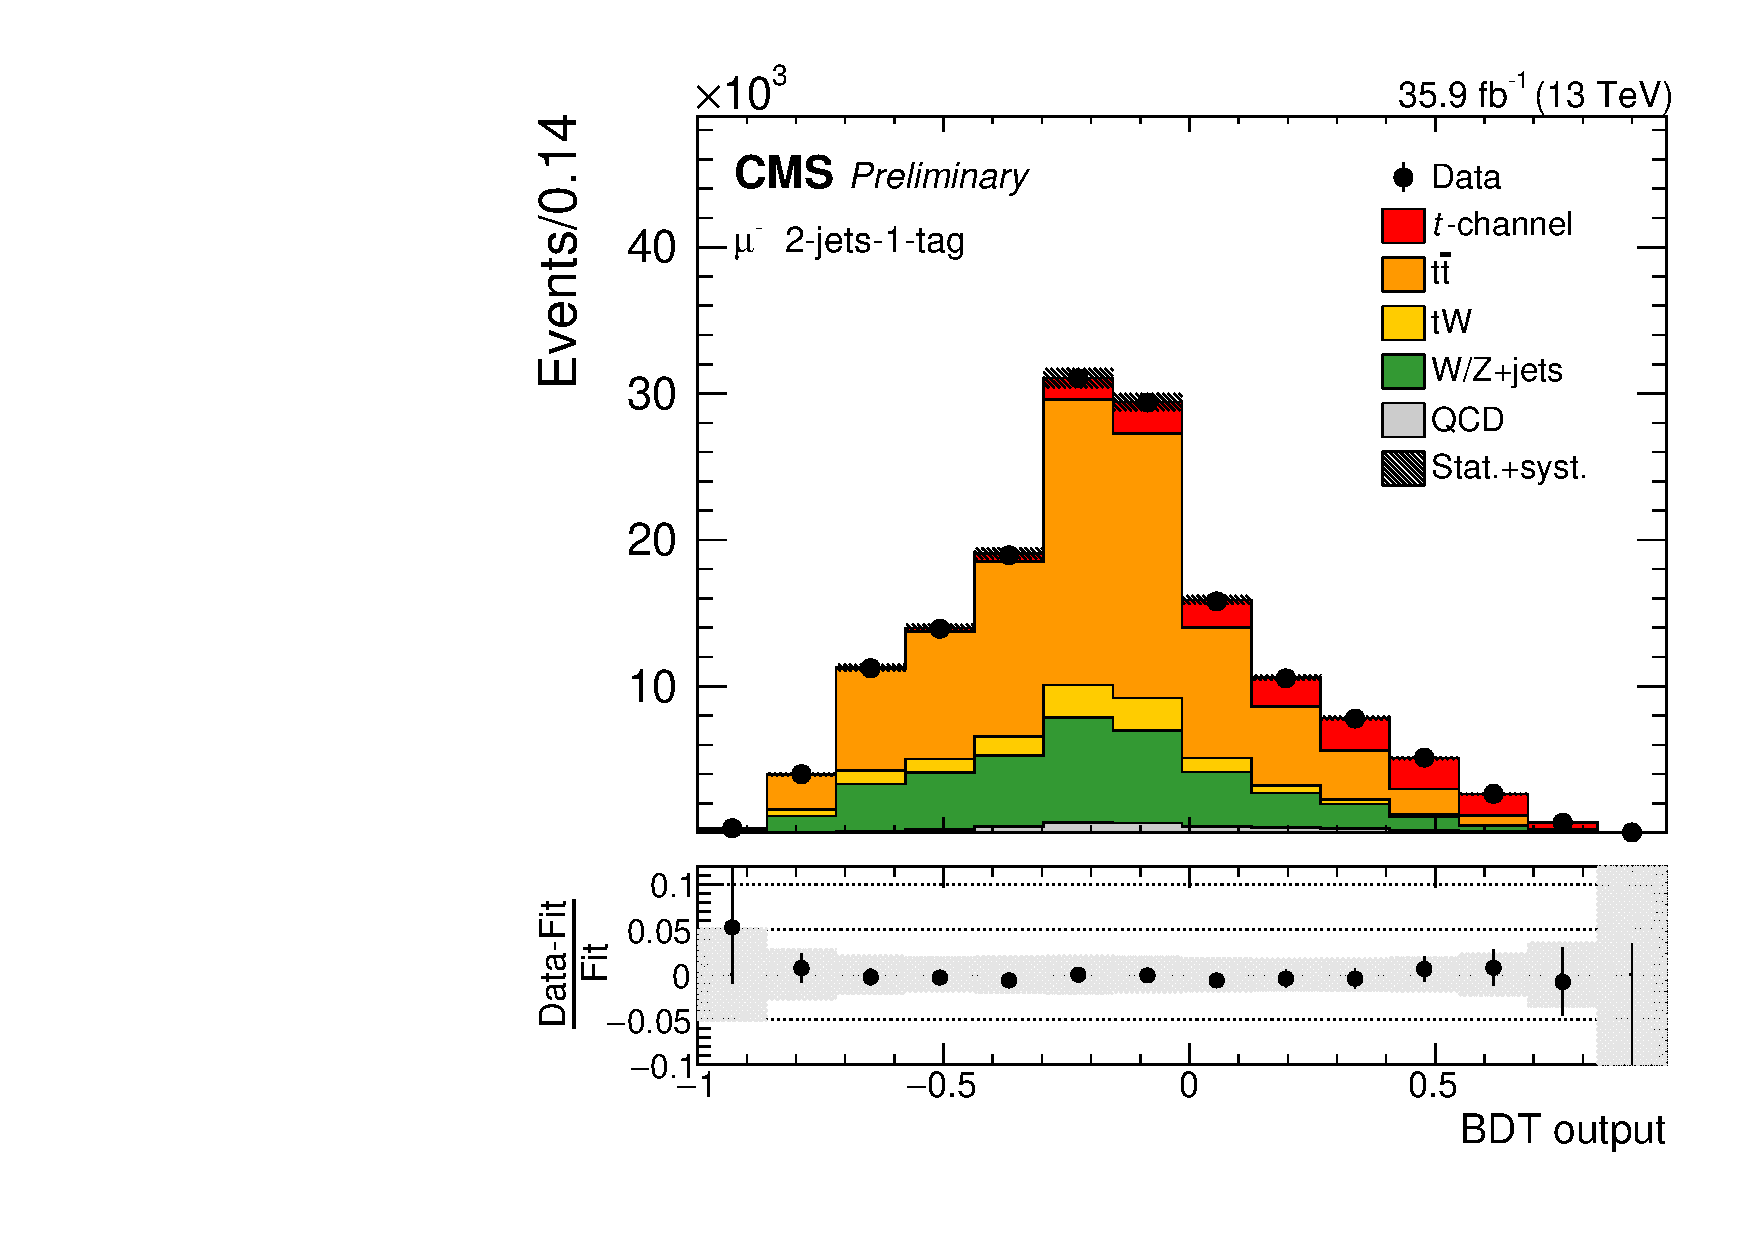
\includegraphics[width=0.48\textwidth]{tch1.pdf}\hspace{0.02\textwidth}
%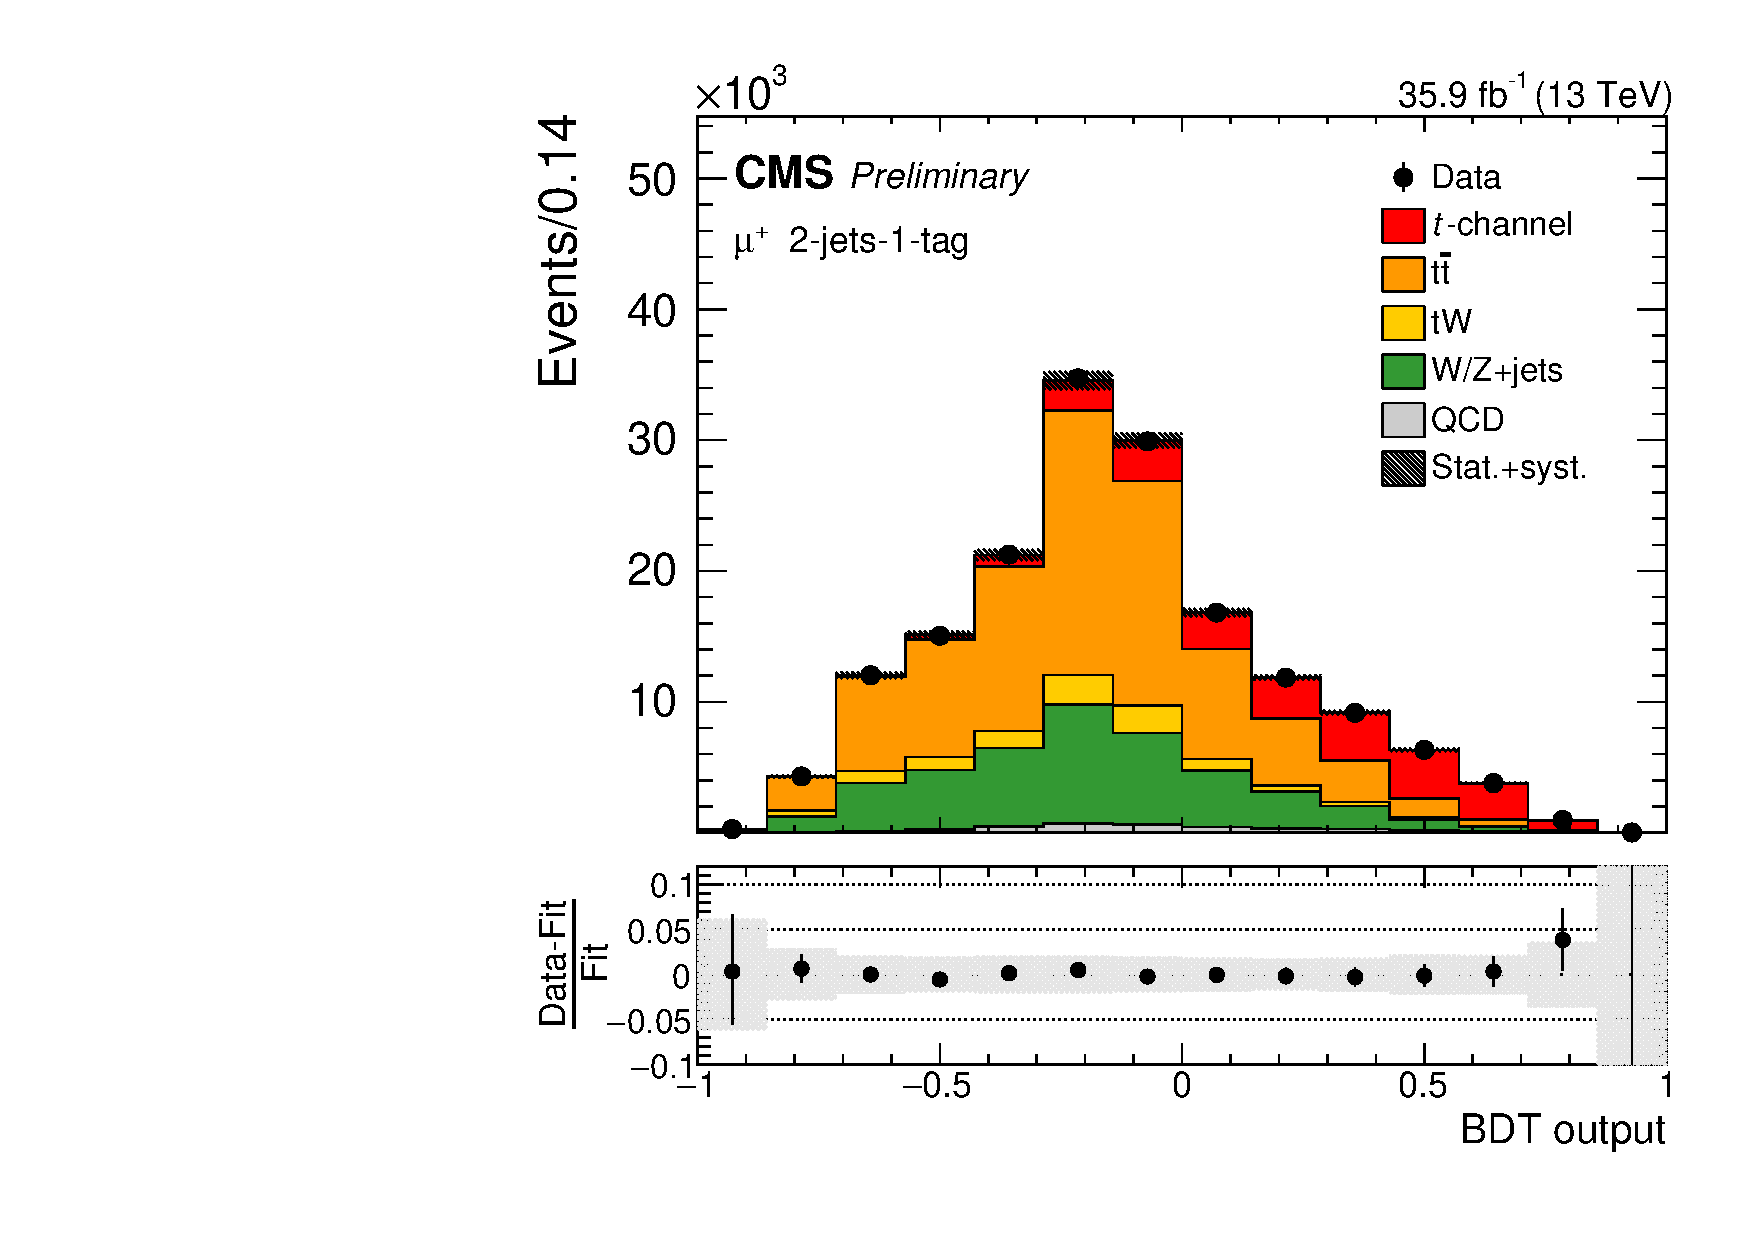
\includegraphics[width=0.48\textwidth]{tch2.pdf}
%\caption{\label{fig:t-channel-bdt}Ref.~\cite{tch}.}
%\end{center}
%\end{figure}

\begin{figure}[!htb]
\begin{center}
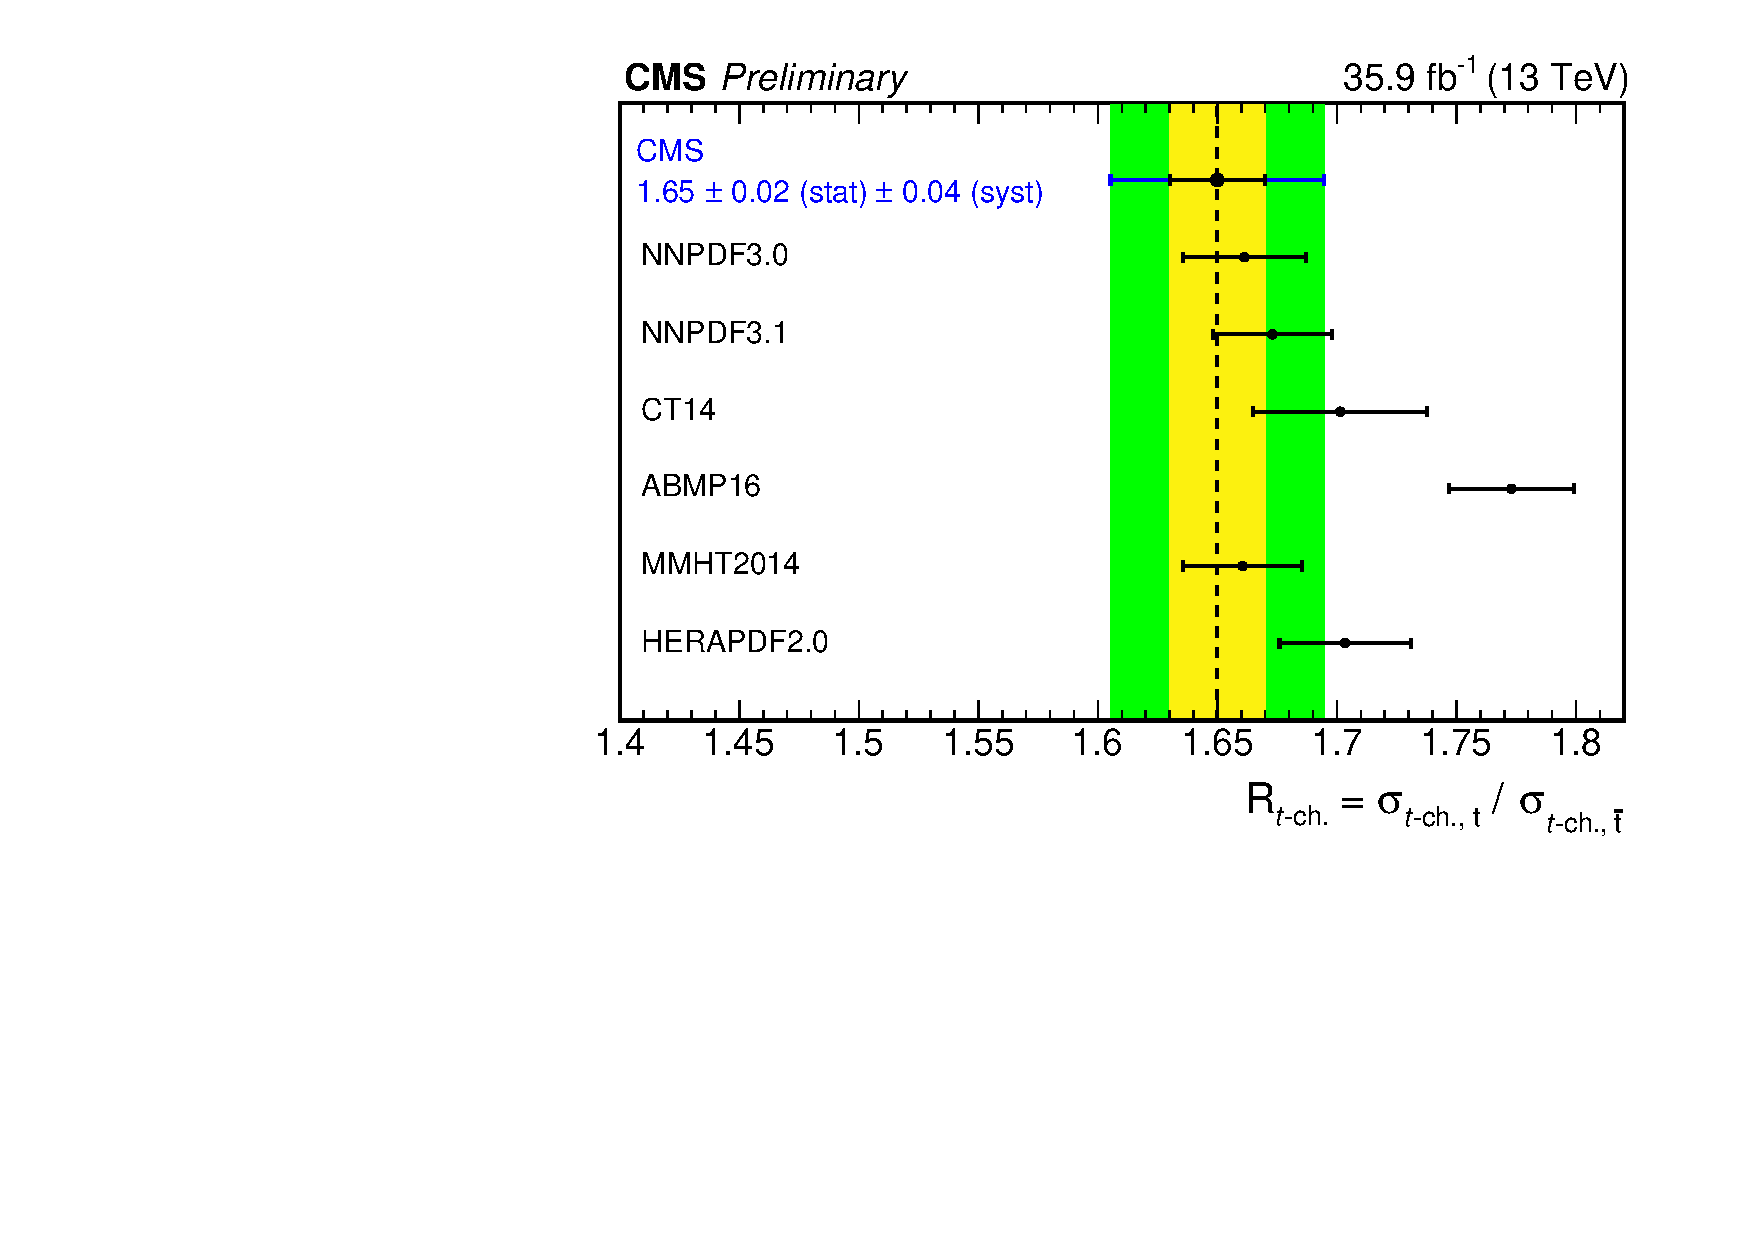
\includegraphics[width=0.6\textwidth]{tch3.pdf}
\caption{\label{fig:t-channel-ratio}Comparison of the measured charge ratio in $t$-channel single top quark production with the predictions by various PDF sets. The figure is taken from Ref.~\cite{tch}.}
\end{center}
\end{figure}

A first measurement of differential single top quark cross sections in the $t$~channel has been performed as well~\cite{tchdiff}. Following a similar event selection as the presented $t$-channel measurement above, the cross section is estimated in intervals of the reconstructed top quark transverse momentum and rapidity through an ML fit to the distribution of a BDT discriminant. The resulting cross sections, shown in Fig.~\ref{fig:t-channel-diff}, are found to be in agreement with the prediction by various generators within uncertainties.

\begin{figure}[!htb]
\begin{center}
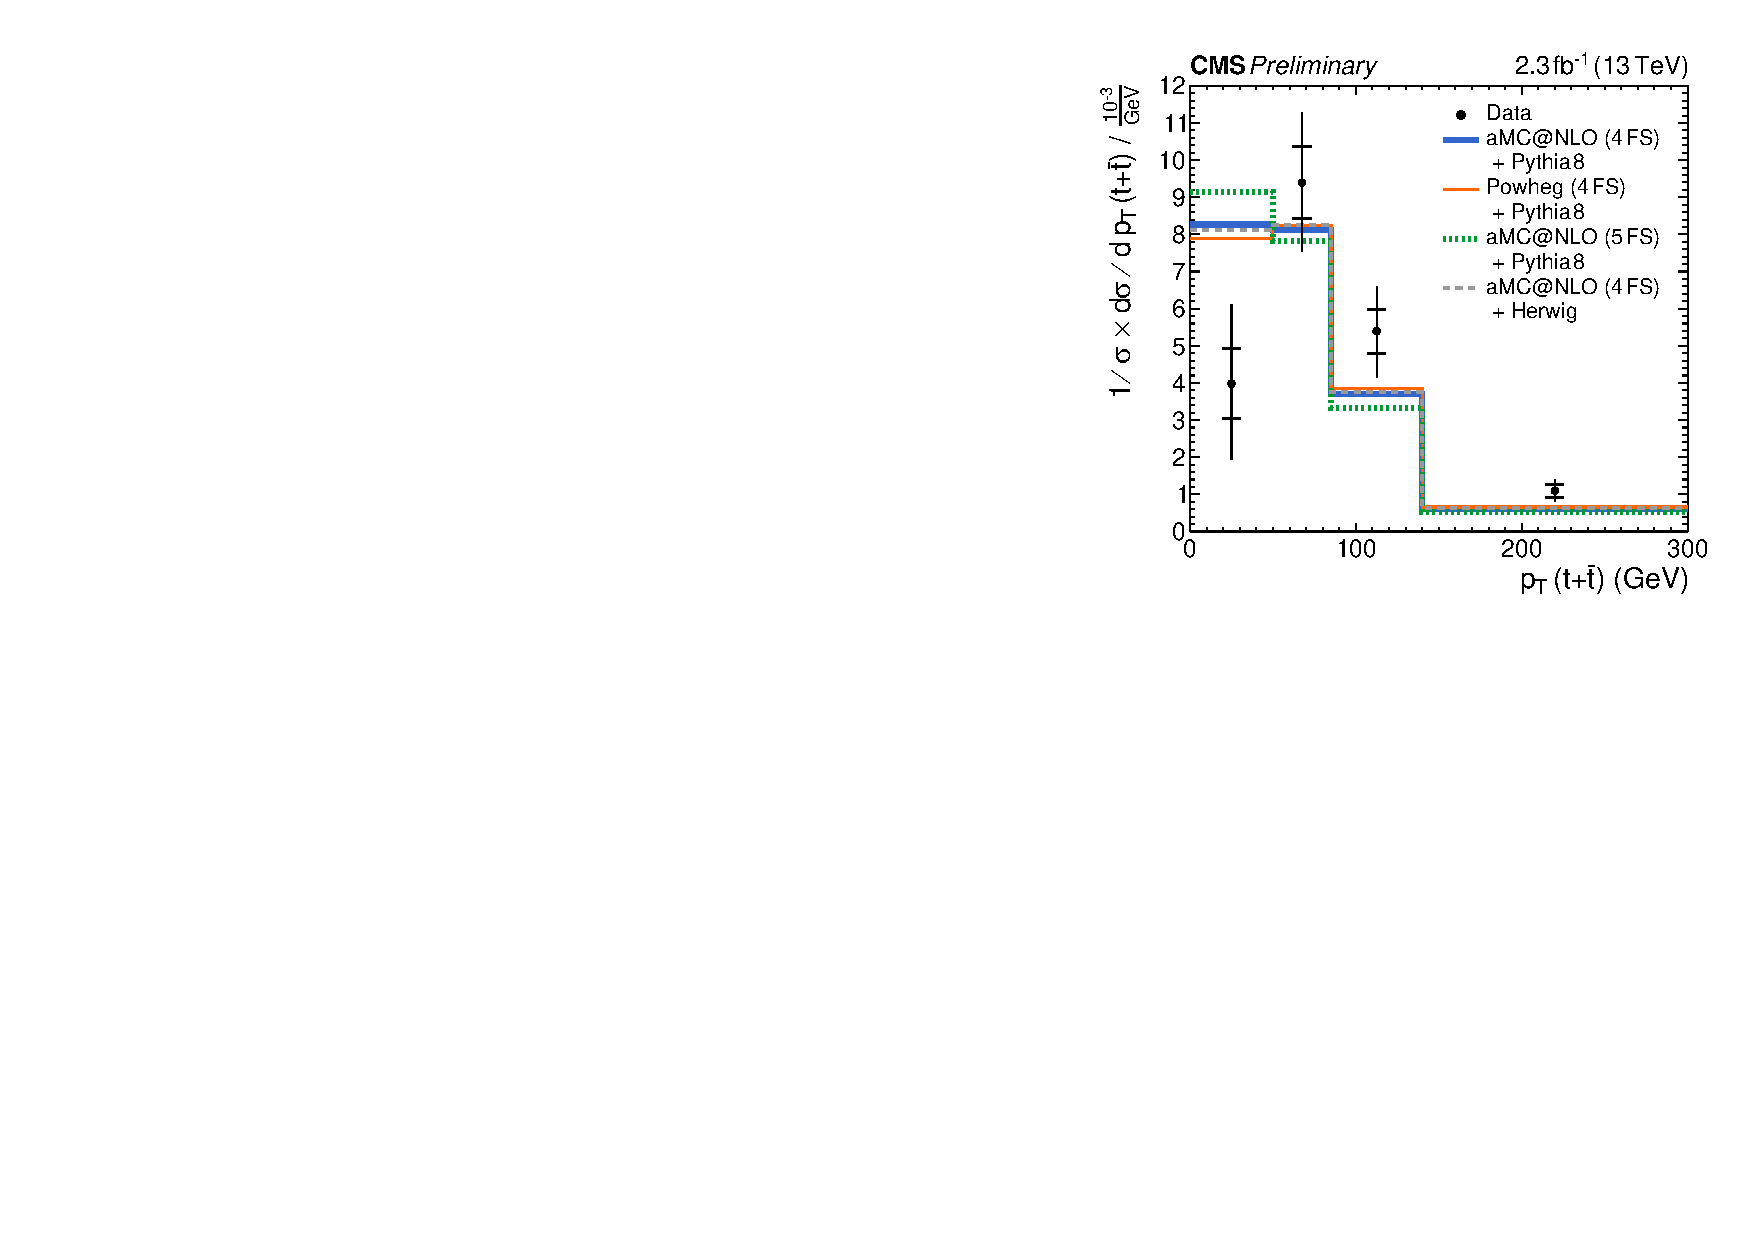
\includegraphics[width=0.48\textwidth]{unfolded_top_pt.pdf}\hspace{0.02\textwidth}
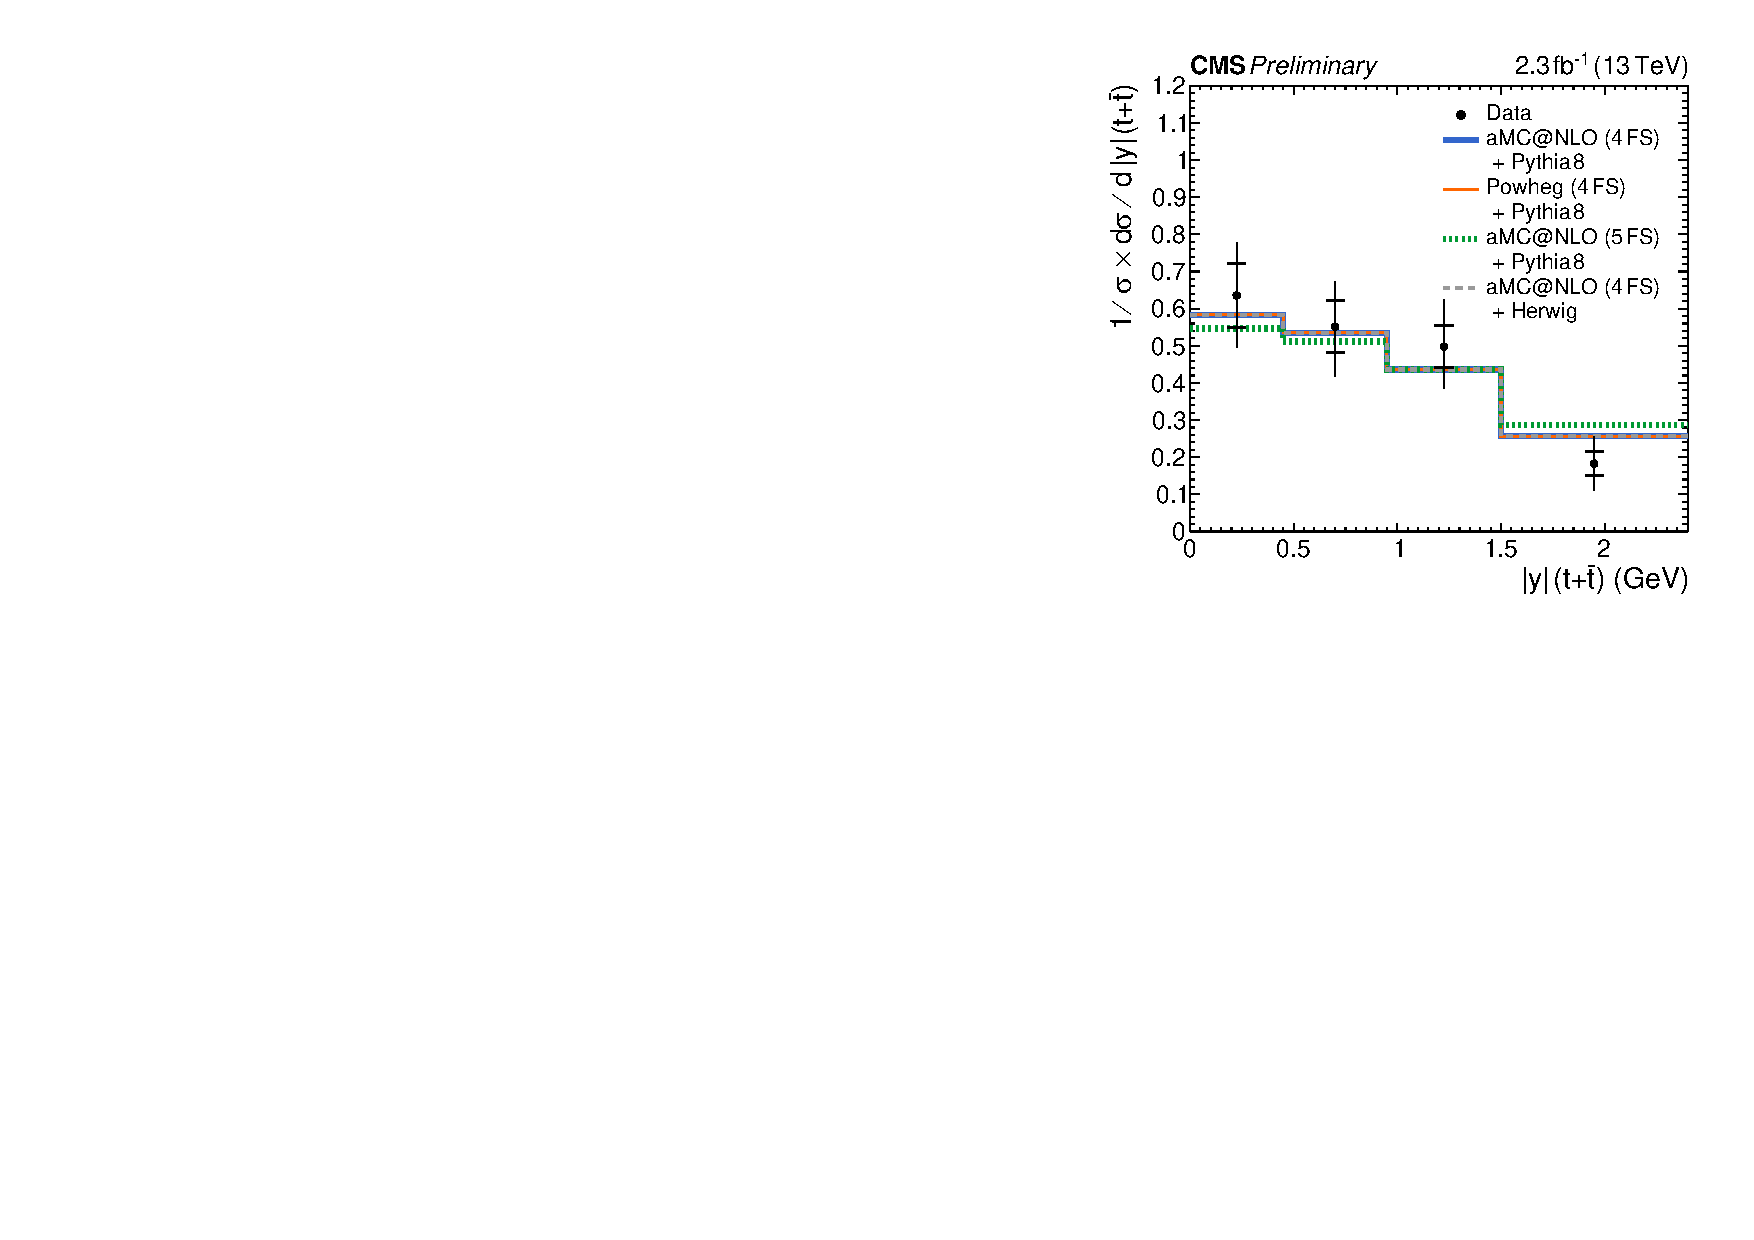
\includegraphics[width=0.48\textwidth]{unfolded_top_y.pdf}
\caption{\label{fig:t-channel-diff}Differential $t$-channel single top quark cross section as a function of (left)~the transverse momentum and (right)~the rapidity of the top quark. The figure is taken from Ref.~\cite{tchdiff}.}
\end{center}
\end{figure}

\section{Conclusion}

Recent measurements of single top quark production in the three main production modes, $s$~channel, W-associated, and $t$~channel, by the CMS collaboration have been presented for which proton-proton collision data recorded at centre-of-mass energies of 7, 8, and 13~TeV have been analysed. Overall the results are found to be in agreement with the predictions.

\begin{thebibliography}{99}

\bibitem{sch}{CMS Collaboration, \emph{Search for s~channel single top quark production in pp collisions at $ \sqrt{s}=$7 and 8~TeV}, JHEP 09 (2016) 027, \texttt{arXiv:1603.02555}.}

\bibitem{tWch}{CMS Collaboration, \emph{Measurement of the production cross section for single top quarks in association with W~bosons in proton-proton collisions at $\sqrt{s}=$13~TeV}, JHEP 10 (2018) 117, \texttt{arXiv:1805.07399}.}

\bibitem{tw-xsec}{N. Kidonakis, \emph{Theoretical results for electroweak-boson and single-top production}, Proceedings PoS DIS 2015, \texttt{arXiv:1506.04072}.}

\bibitem{tch}{CMS Collaboration, \emph{Measurement of the single top quark and antiquark production cross sections in the t~channel and their ratio in pp collisions at $\sqrt{s}=$13~TeV}, CMS-PAS-TOP-17-011, 2018, \texttt{cds.cern.ch/record/2628541}.}

\bibitem{hathor}{P. Kant, et al., \emph{HATHOR for single top-quark production: Updated predictions and uncertainty estimates for single top-quark production in hadronic collisions}, Comput.Phys.Commun. 191 (2015), \texttt{arXiv:1406.4403}.}

\bibitem{tchdiff}{CMS Collaboration, \emph{Measurement of the differential cross section for t-channel single-top-quark production at $\sqrt{s}=$13~TeV}, CMS-PAS-TOP-16-004, 2016, \texttt{cds.cern.ch/record/2151074}.}

\end{thebibliography}



\end{document}
